In the supplementary materials, we provide the construction of the training set in \cref{TrainingSet}, and present more experimental setup and results in \cref{Experiments_Results}. We strongly recommend viewing the static HTML files in the supplementary materials for a direct and clear demonstration of the unique capabilities of our model and significant improvements over previous methods.



\section{Construction of the Training Dataset}
\label{TrainingSet}

Our training datasets are all open-source datasets, primarily including open-source image personalization datasets and open-source video personalization datasets. Specifically, image personalization datasets consist of four parts: UNO \cite{UNO}, Echo-4o \cite{echo-4o}, MUSAR \cite{musar}, and Nano-Consistent-150K \cite{echo-4o}. UNO and Nano-Consistent-150K are single-subject datasets, and the remaining datasets are multi-subject datasets. We primarily filter the datasets based on aesthetic quality and personalization quality scores using an MLM-based evaluation system, ultimately obtaining 200K high-quality image datasets to enable text-to-video models with basic personalization ability. The video personalization datasets we use are also all open-source datasets; the number of samples after filtering for each dataset is shown in Tab. \ref{tab:datasets}.





\begin{table}[ht]
  \caption{Detailed description of the training dataset.}
  \label{tab:datasets}
  \centering
  \resizebox{0.85\textwidth}{!}{
  \begin{tabular}{@{}cccc@{}}
    \toprule
    Dataset Name & Filtered Dataset Size & Modality & Category  \\
    \midrule
    UNO \cite{UNO} & 50K & Image & Single Subject  \\
    Nano-Consistent-150K \cite{echo-4o} & 60K & Image & Single Subject \\
    Echo-4o\cite{echo-4o}  & 60K & Image & Multi Subject \\
    MUSAR\cite{musar} & 30K & Image & Multi Subject \\
    Total Dataset & 200K & Image & - \\
    \midrule
    Phantom-Data\cite{phantom-data} & 400K  & Video & Single \& Multi Subject \\
    Opens2v\cite{yuan2025opens2v} & 300K & Video & Multi Subject \\
    Ditto-1M\cite{ditto1m} & 50K & Video & Single \& Multi Subject \\
    Total Dataset & 750K & Video & - \\
  \bottomrule
  \end{tabular}}
\end{table}



\begin{figure*}[h]
    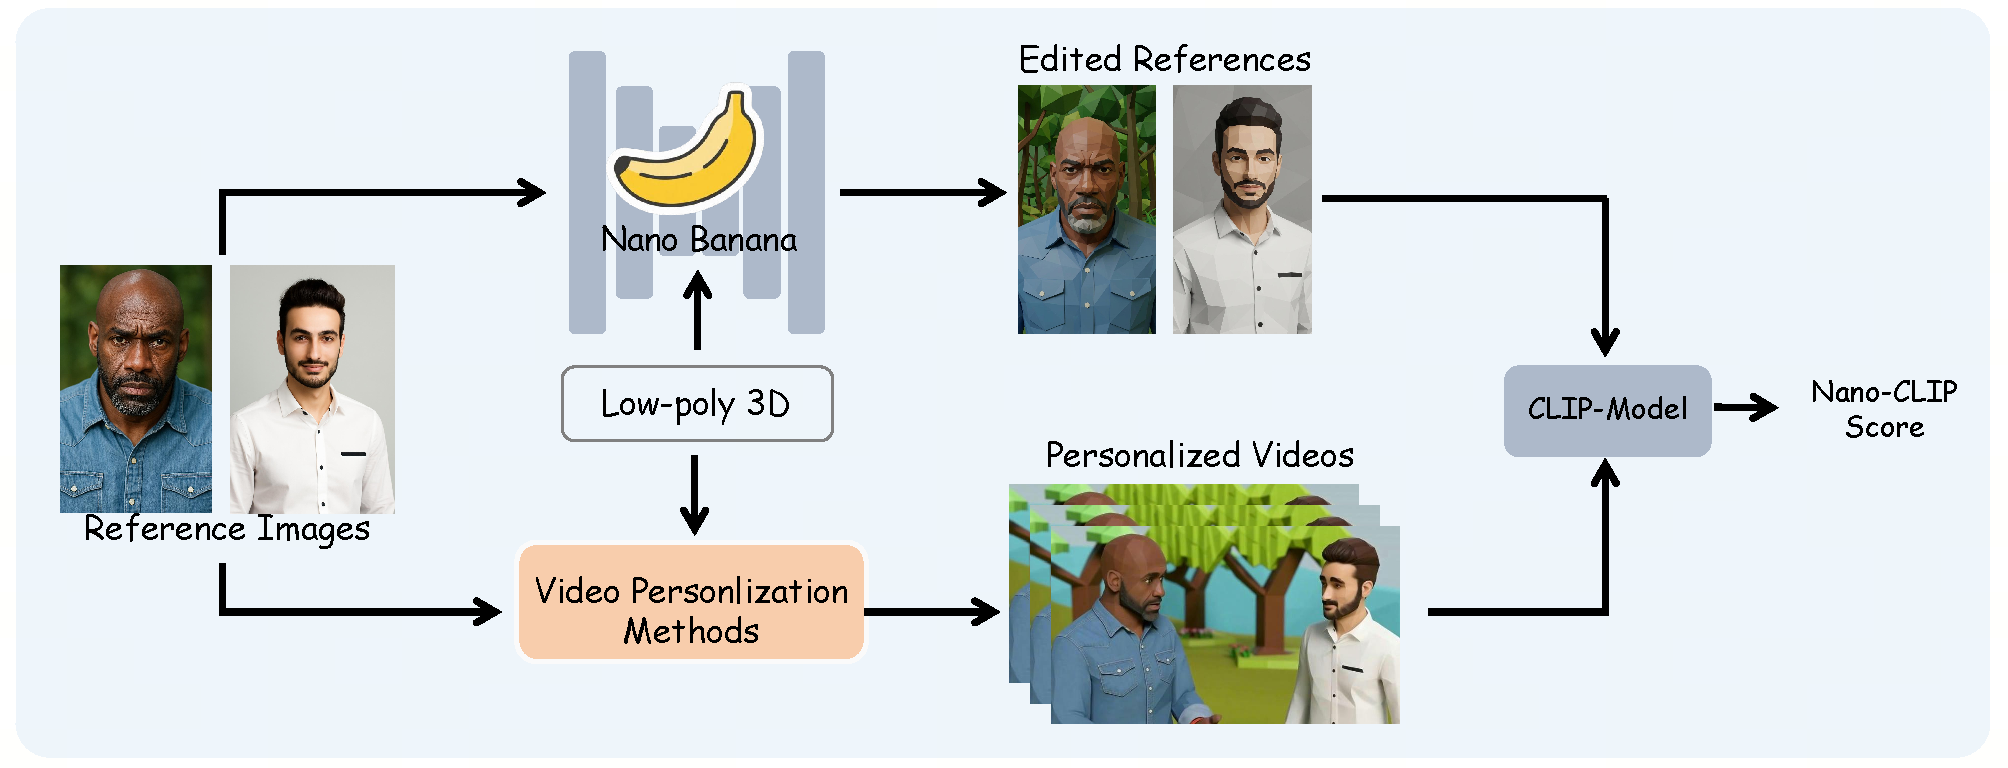
\includegraphics[width=0.98\linewidth]{figures/nano_clip_pipeline.pdf}
    \caption{The calculation process of the Nano-CLIP metric. Given reference images and a domain transformation prompt, Nano Banana Pro first generates edited reference images. Each video personalization method then generates videos conditioned on the prompt. Finally, CLIP computes the cosine similarity between the generated frames and the edited references. The average similarity across frames is used as the Nano-CLIP score. Qwen-CLIP follows the same pipeline, except that the image editing model is replaced with Qwen-Image-Edit.
}
    \label{fig:nano}
\end{figure*}

\begin{table*}[!t]
\centering
\caption{MLLM prompt for Cross-Domain (CD) Score and Qwen-Score.}
\label{tab:cd score}
\resizebox{1.0\textwidth}{!}{%
\begin{tabular}{p{0.95\textwidth}}
\toprule
Guidelines: You are an experienced AI evaluator for cross-domain subject-driven text-to-video generation. You will receive two images and a reference caption.\\
\midrule
Reference Image 1: a reference subject. \\
Image 2 from Generated Video: the subject in a cross-domain scenario. For example, a person from the real world domain is transformed into a fantasy character, or an anime character is transformed into a real-world doll. \\
Reference Caption:  describes the intended subject and scene.
\\ \\
Task: \\
Your task is to measure the performance of transforming reference image 1 to image 2 based on the reference caption and the intrinsic features of reference subjects (\eg, shape, color, texture, and appearance). \\

\midrule

Scoring Rules: \\
1. Assign a score between 1 and 5. \\
2. Metric: \\
         \hspace{1em}  \textbf{5}: Achieving good cross-domain transformation while preserving the most features in reference image 1; \\
         \hspace{1em} \textbf{4}: Achieving cross-domain transformation of key features in reference image 1, but some negative and non-critical feature transformations have flaws. \\
        \hspace{1em} \textbf{3}: Achieving cross-domain transformation for part key features (such as human body), but domain transformation is not achieved for the remaining key and minor features. \\
         \hspace{1em} \textbf{2}: Only achieving the transformation of some negative and non-critical features in reference image 1, such as background and minor decorative elements, while the transformation of key features (e.g., human face) fails. \\
         \hspace{1em} \textbf{1}: Almost completely copies and pastes the features of reference image 1 without any cross-domain transformation. Alternatively, the cross-domain transformation result completely discards the features of reference image 1. \\ \\
3. Higher scores correspond to higher cross-domain consistency. \\
Strict Output Requirement: Return only the numerical score (no explanations, text descriptions, or additional comments).  \\
 \bottomrule
\end{tabular}%
}
\end{table*}


\begin{table*}[!t]
\centering
\caption{Guidelines of human preference evaluation.}
\label{tab:user_study}
\resizebox{1.0\textwidth}{!}{%
\begin{tabular}{p{0.95\textwidth}}
\toprule
Guidelines: Open-Domain subject-driven video (S2V)  personalization is an important downstream task of text-based video generation, aiming to generate videos based on user-provided images and prompts.  Open domain S2V mainly involves two scenarios: in-domain (\eg, multi-human, multi-object, and human-object interaction) scenarios and cross-domain (\eg, real-world subject to fantastic domain, fantastic subject to real-world domain, and the interaction of the real-world and fantastic subjects) scenarios. Please watch the following randomly selected videos, reference images, and prompts. Compare their effects and evaluate the generated video based on three metrics: \\


\midrule
1. Overall Video Quality: Comprehensively evaluate the overall quality of the generated videos from three aspects: aesthetic quality, the smoothness of subject motions (avoiding static or frozen subjects and frame discontinuities), and the naturalness of color, texture, and saturation. \\

 \\
 
2. Evaluate text controllability based on the consistency between the generated video and the input text description (\eg, corresponding real-world or fantastic domain descriptions, stylistic attributes, and subject interaction alignment). \\

\\

3. Open-Domain Subject Consistency: Evaluate subject consistency based on the similarity between the generated subject and the subject of the reference images. In in-domain scenarios, the best methods require retaining the reference subject features as much as possible. In cross-domain scenarios, the best methods should preserve the intrinsic features of the subject (\eg, hairstyle, skin color, and clothing) while allowing subject-irrelevant properties (\eg, lighting, style, and domain attributes) to vary flexibly according to the text prompt.  \\
\midrule

Please rank these methods across these three metrics. \\
 \bottomrule
\end{tabular}%
}
\end{table*}


\section{More Experiments Results}

\label{Experiments_Results}

\subsection{Implementation Details}

\textit{DomainShuttle} utilizes the default settings for inference for both Wan2.1 and Wan2.2, using 50 sampling steps on Wan2.1 and 40 steps on Wan2.2. The classifier-free guidance scale is set to 3 in Wan2.1. In Wan2.2, the high-noise classifier-free guidance scale is set to 4, while the low-noise guidance scale is set to 3. All flow shift parameters are set to 5.



\subsection{Evaluation Details}

\paragraph{\textbf{Evaluation Dataset.}} The 110 in-domain testset includes 90 \textbf{open-source} cases from OpenS2V-Eval \cite{yuan2025opens2v}, with 30 each for multi-human, multi-object, and Hard\_dev cases. Because some methods support at most four subjects, we use the first four subjects in each Hard\_dev case as references. Additionally, the in-domain test set includes 20 human–object interaction cases. For the cross-domain evaluation dataset, we construct 40 multi-subject samples for real-world subjects in fantasy domains, 40 multi-subject samples to map the fantasy subjects to the real-world objects, and 30 multi-subject samples for interactions between real-world and fantastic subjects.




\paragraph{\textbf{Evaluation Metrics.}} For all subject similarity metrics, we uniformly sample 16 frames from the videos generated by each method, compute the score for each frame, and take the average score as the final result.

The evaluation process of Nano-CLIP is shown in Fig. \ref{fig:nano}. For the Nano-CLIP metric, we first use Nano Banana Pro \cite{nano_banana} to generate the edited reference images based on the reference images and the domain transformation prompt. Next, guided by the prompt, each video personalization method generates videos of the reference images. Finally, CLIP is used to calculate the cosine similarity between each frame of the generated videos and the reference images edited by Nano Banana. The average similarity across all frames is used as the Nano-CLIP score for these methods.

The Cross-Domain Score leverages the comprehensive understanding capability of the multimodal large language model (\ie, GPT-5.2) to thoroughly evaluate the intrinsic subject consistency of different methods in cross-domain scenarios. Detailed evaluation instructions are provided in Tab. \ref{tab:cd score}. We average all scores and apply normalization to obtain the final results.




\subsection{Evaluation Criteria for Human Preference Evaluation}



Each volunteer is presented with 20 randomly selected open-domain videos for our method and four strong baselines, resulting in 100 videos in total. For each group, participants are required to rank the videos under every metric, assigning scores from 5 (best) to 1 (worst). Ties are not allowed in any ranking for any metric. The instructions provided to the participants are shown in Tab. \ref{tab:user_study}.



\subsection{More Qualitative Comparisons.}

We present more qualitative comparisons between \textit{DomainShuttle} and the baselines in the supplementary materials, as shown in Fig. \ref{fig:visual_case_5} and  Fig. \ref{fig:visual_case_6}. Our method outperforms existing methods across all three scenarios: mapping real-world subjects to fantasy domain, mapping fantasy subjects to the real world, and interactions between fantasy and real-world subjects. These qualitative comparisons demonstrate that \textit{DomainShuttle}  can achieve flexible text controllability and precisely preserve the intrinsic features of the reference subject.

\subsection{More Ablation Study}

In addition, we conducted an ablation study on whether to use Ditto-1M, as shown in the Tab. \ref{video_editing}. Without Ditto-1M,  our method remains effective and still achieves cross-domain SOTA performance, improving the CD-Score by 13.5\% over baselines (0.725 of Kling 1.6).


\begin{table*}[t]
\centering
\caption{\textbf{Ablation Studies} of Ditto 1M. }
\renewcommand{\arraystretch}{1.15}
\small
\begin{tabularx}{\textwidth}{l *{4}{>{\centering\arraybackslash}X}}
\toprule
Method (Wan 2.2) & NANO-CLIP $\uparrow$ & CD-Score $\uparrow$ & DINO-I $\uparrow$ & CLIP-I $\uparrow$ \\
\midrule
w/o Ditto 1M & 0.631 & 0.823 & \textbf{0.432} & \textbf{0.701} \\
w Ditto 1M   & \textbf{0.636} & \textbf{0.861} & 0.400 & 0.690 \\
\bottomrule
\end{tabularx}
\vspace{-6pt}
% \caption{Comparison on video editing benchmark.}
\label{video_editing}
\end{table*}


\begin{figure*}[!t]
    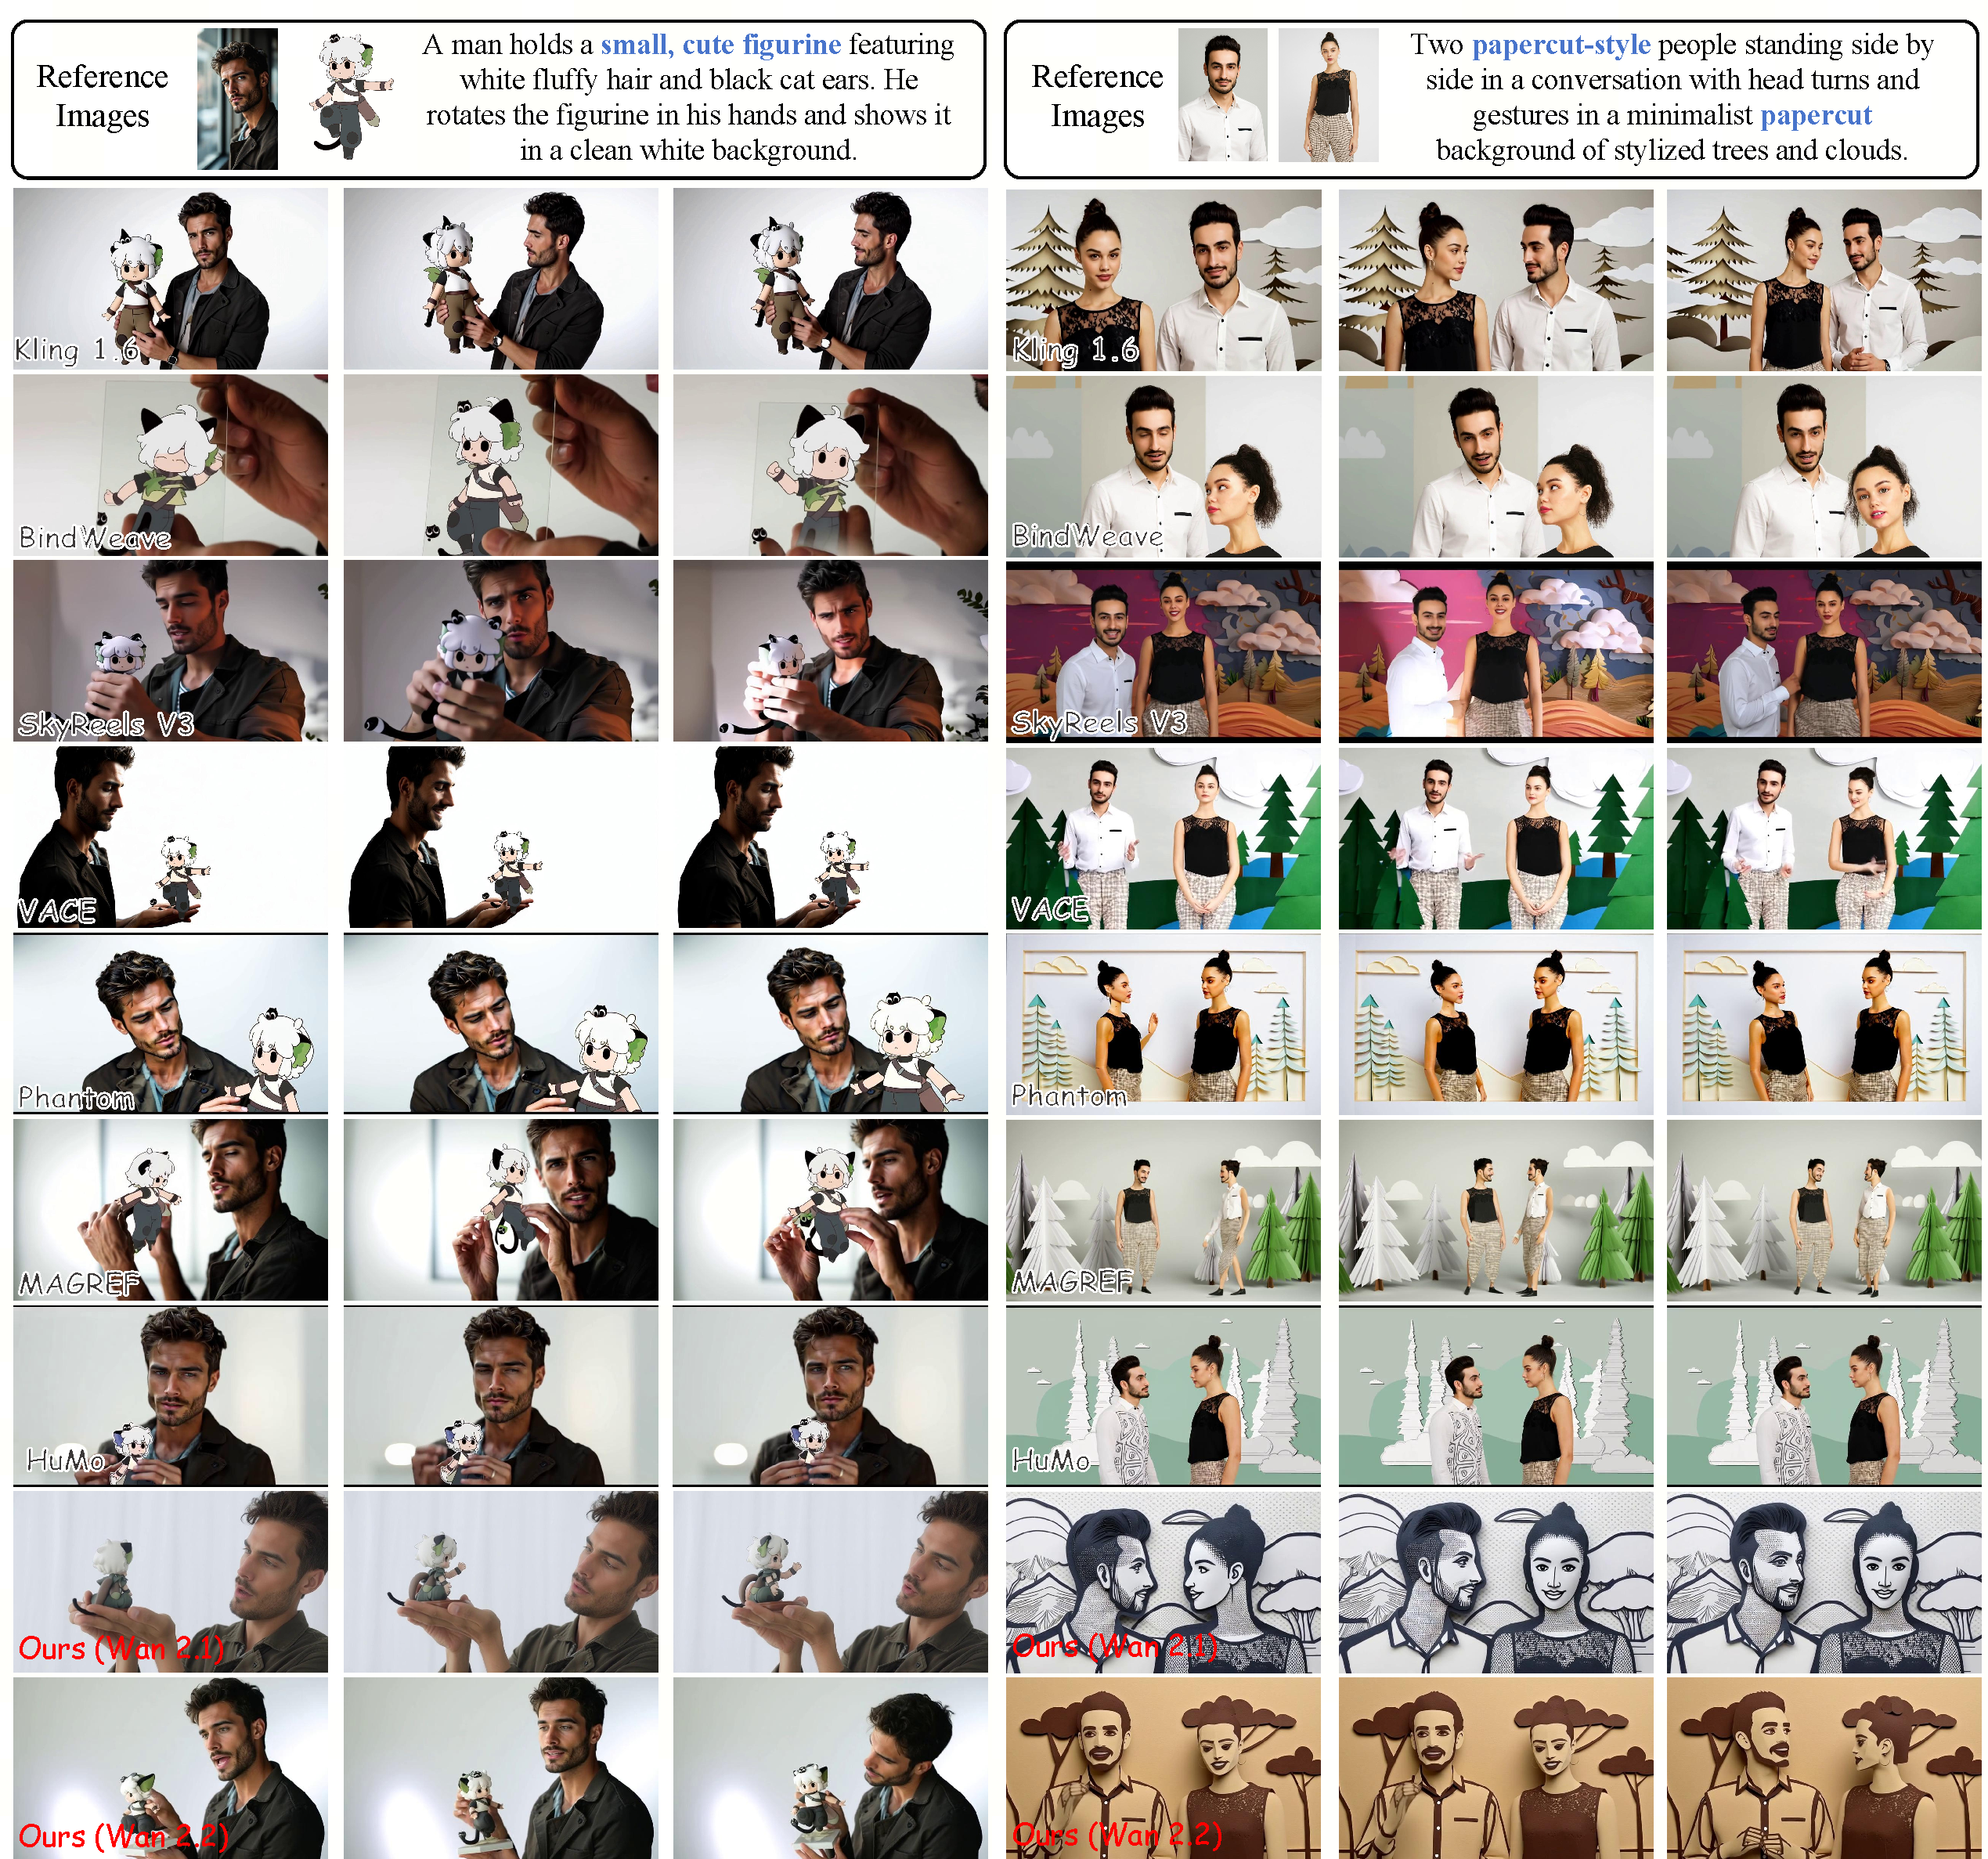
\includegraphics[width=0.98\linewidth]{figures/visual_case_5.pdf}
    \caption{\textbf{More qualitative comparison} with existing methods. For mapping fantasy-domain subjects to real-world subjects, \textit{DomainShuttle} successfully converts the fantasy character into a real-world small figurine, outperforming existing methods. For real-to-fantasy, \textit{DomainShuttle} transforms real-world subjects into the corresponding paper-cut fantasy domain, whereas existing methods fail to achieve this conversion.
}
    \label{fig:visual_case_5}
\end{figure*}


\begin{figure*}[!t]
    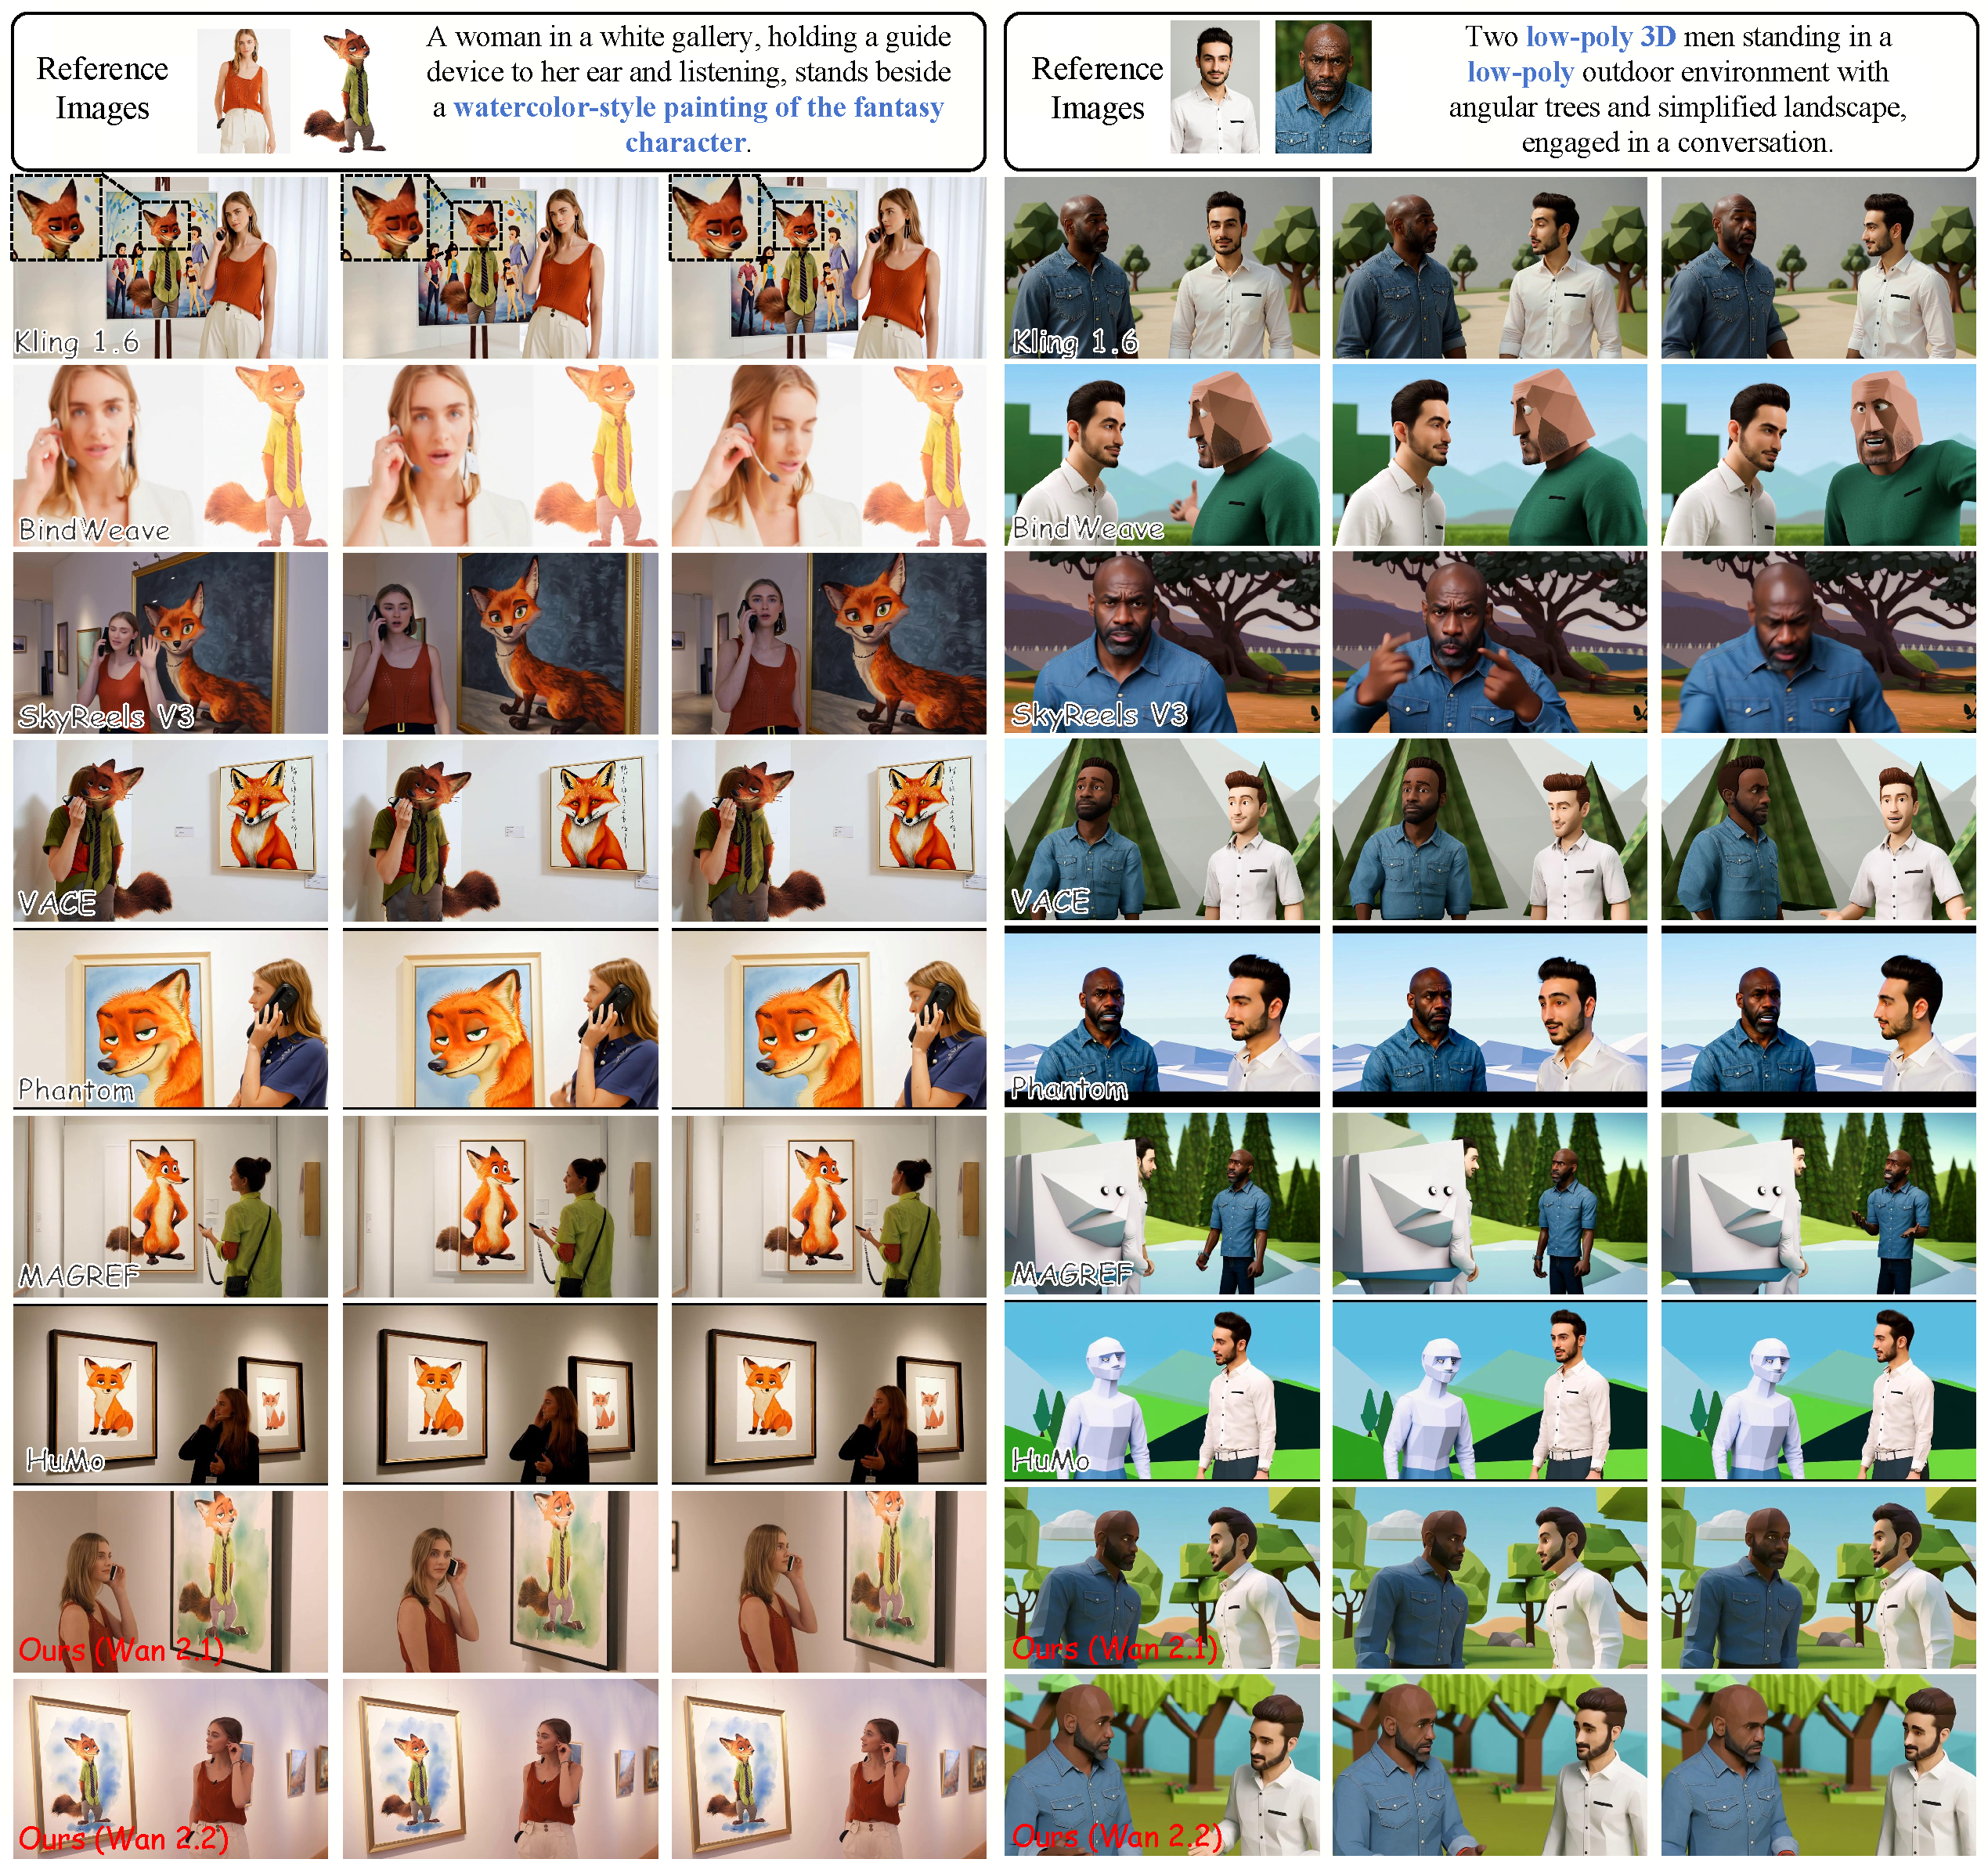
\includegraphics[width=0.98\linewidth]{figures/visual_case_6.pdf}
    \caption{\textbf{More qualitative comparison} with existing methods. For real–fantasy subject interactions, \textit{DomainShuttle} successfully generates interactions between the woman and the painting of the fantasy character. Among existing methods, the commercial model Kling-1.6 performs comparatively well, but the painted character blinks, which contradicts the static nature of the painting. For real-to-fantasy scenario, our method accurately maps real-world subjects to the low-poly 3D domain. In contrast, existing methods either fail to transfer subjects or lose key subject features after transfer.}
    \label{fig:visual_case_6}
\end{figure*}
